\title{G54MRT Coursework 1 - \emph{Walking In Wollaton}}
\author{}
\date{}
\documentclass[12pt, a4paper]{article}

\usepackage{graphicx}
\graphicspath{{Images/}}

\begin{document}
\maketitle

\section{Design Sketch}
\subsection{Summary}
The objective of the game is to encourage users to explore all areas of Wollaton Hall, and by extension Wollaton Park.
The game will aim to take a user on a "guided tour" of the grounds by providing the user with a series of "collectables" relating to exhibits in the museum that makes up Wollaton Hall, and some of the surrounding landmarks such as Wollaton Park Lake.
These areas will be defined based on the map in Figure \ref{fig:wollatonmap}.

\begin{figure}[ht]
  \centering
  \caption{A map of the Wollaton Park grounds, taken from www.wollatonhall.org.uk/visit}
  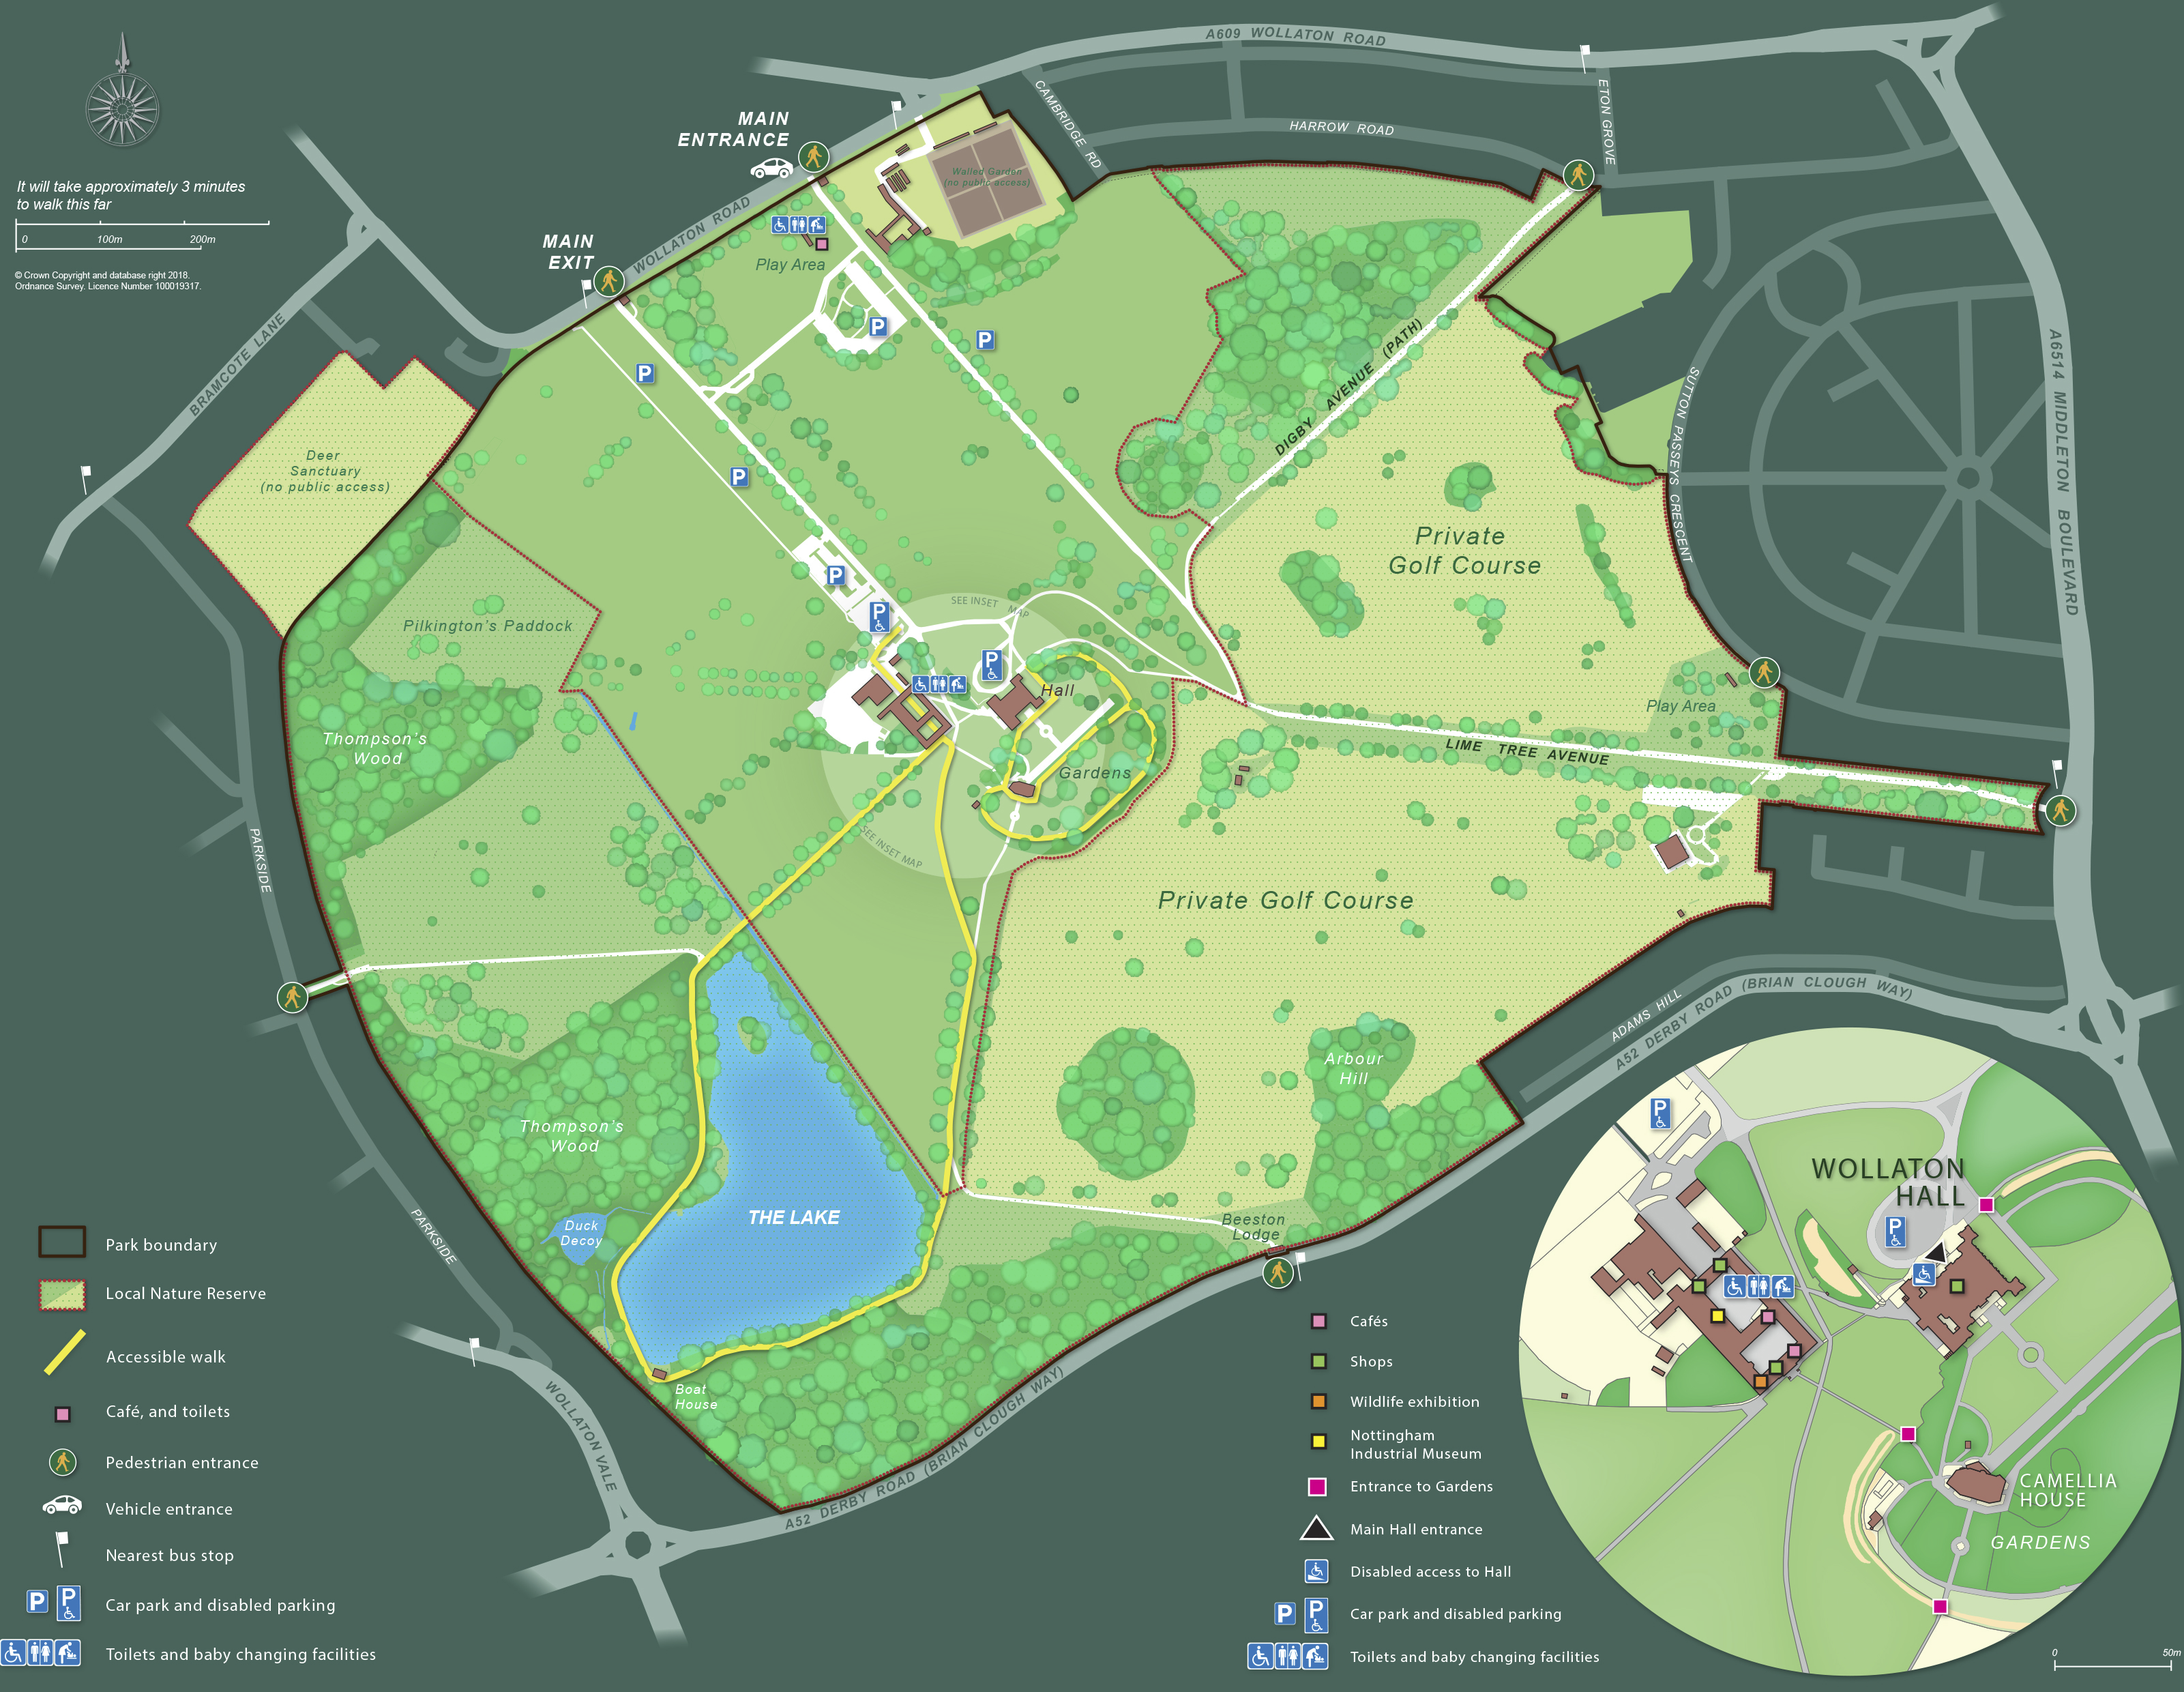
\includegraphics[width=\textwidth]{wollaton-park-map.png}
  \label{fig:wollatonmap}
\end{figure}

The main consideration that should be taken here is that users do not stray onto either the deer sanctuary in the northwest corner or the golf course that makes up much of the southeast of the park.
The game will be prototyped using the WanderAnywhere platform, mainly because it will be more of the form of a "walking simulator" a la \textit{Dear Esther}.

\subsection{Ideation Cards}
I will take 3 ideation cards from each category and in the following section outline my responses to them.

\subsubsection{Opportunities}
\begin{itemize}
  \item Scavenger Hunt - Players travel between locations to find clues or treasures\\
        The whole objective of the game is that players move between locations and "collect" treasures in the form of experiences.
  \item Unusual Locations - Players get to visit places they otherwise would not\\
        Again, the nature of the game is such that it will hopefully encourage people to explore a greater area of the Park grounds than they otherwise would, and potentially even parts of the museums on said grounds that they would ordinarily ignore.
  \item Exergaming - The game requires acts of endurance, strength, or dexterity\\
        The gamification aspect of the experience means that a user could be scored on how long it takes them to "collect" a set number of objectives - this may mean visiting 8 unique areas and the fastest time wins.
        In a more realised version of the game it may be preferable that the game become social, and that a group of users select the locations to explore and race one another.
\end{itemize}

\subsubsection{Questions}
\begin{itemize}
  \item Duration - How long is a game session? Should it be shorter or longer?\\
        The duration of the game is the scoring system in a sense, so this aspect will refer to the number of objectives to be explored before a session is considered finished.
        Ideally the game will take no more than a couple of hours to finish at a leisurely pace, although speedrunners exist for all forms of video game.
  \item Experience Flow - How do players journey through the game?\\
        The users will journey from point to point around the park, likely staying to the west of the house given that the east is made up mostly of the golf course, a play area, and a walled garden to which the public has no access.
  \item Indoor / Outdoor - Can the game be played in both? Should it? What would change?\\
        By its nature the game will be played in both, although given a larger museum it could be adapted to be entirely indoors.
        I feel that the dual nature of the game will ultimately make it more enjoyable - with potential for different game modes including an entirely indoors version for less weather-conducive days.
\end{itemize}

\subsubsection{Challenges}
\begin{itemize}
  \item Long Distances - How are players engaged while between game locations?\\
        This is in my view the greatest challenge the game will face, and will depend greatly on the chosen path between objectives.
        Ideally the game will provide information about the history of the grounds or information on local wildlife in between locations, however this may be redundant if some of the objectives relate to those topics.
  \item Phone Zombies - Will players be staring at their screens most of the time?\\
        Again this is a matter of the design of the game at the "in-between" phase, as at each point the game should be set up such that it encourages the user to not look at their screens until it is time to go to another location.
  \item Unstable Connectivity - How does the game continue without a data connection?\\
        The full version of the game should contain locally all of the required information for the game to continue sans data.
\end{itemize}

\subsection{Concept Sketch}

\section{Photostory}

\section{Testing}
\subsection{Testing Process}
\subsection{Issues Revealed}

\section{Critical Reflection}


\end{document}

